% Chapter 2

\chapter{Conclusiones} % Main chapter title

\label{Conc} % For referencing the chapter elsewhere, use \ref{Chapter2} 

Se diseñó e implementó un sistema de navegación capaz de conocer su ubicación en un entorno geográfico con una alta precisión para apoyar en proyectos que requieran de una alta confianza de datos de geolocalización, utilizando dispositivos pequeños y portátiles para no sacrificar la movilidad de, en este caso, un vehículo aéreo no tripulado. El \textit{rover} puede funcionar en forma mínima solo con una BeagleBone Black, el dispositivo GPS y el dispositivo convertidor de RS232 a Serial TX-RX en valores lógicos CMOS.\\

Para realizar la tarea anterior de una forma más sencilla, se utilizaron sistemas de archivos en red o NFS entre la BeagleBone Black y una PC con GNU/Linux para compartir un directorio donde, por ejemplo, podían depurarse errores en los códigos sin necesidad de realizar transferencias mediante ssh de una forma extensiva. Previo a eso, a la PC se le instaló un emulador de Debian con arquitectura ARM para que los programas compilados puedan ser interpretados correctamente por la BeagleBone Black.\\

Se realizaron diversos circuitos en donde se colocaron los distintos periféricos, explicados en el capítulo de diseño del hardware y del software\ref{Chap:DisHard}. Se realizaron pruebas de desempeño y, una vez funcionando de la forma esperada y sin errores, se soldaron en placas fenólicas junto a cables de bus de datos para una mejor organización del cableado.\\

Durante la programación, se utilizó C++ para crear las bibliotecas que manejaran todos los periféricos, así como el programa principal, quien invocaría al resto de programas necesarios e instanciaría los objetos necesarios.\\

También se entabló una comunicación inalámbrica utilizando el protocolo ZigBee y dos dispositivos XBEE en configuración de par, donde uno emitiría los datos de posicionamiento y otro recepcionaría dichos datos y los comunicaría a la BeagleBone en el caso de que los GPS utilizados no contaran con comunicación inalámbrica integrada.\\ 

Durante la realización de este trabajo de tesis, se realizaron diversos experimentos en donde se logró identificar la mayor estabilidad otorgada por Real-Time Kinematics a comparación de un modo donde el GPS funciona sin retroalimentación. Dichas observaciones fueron corroboradas durante la realización del experimento. Por ejemplo, en la figura~\ref{fig:Pruebas} se puede observar la consistencia de una ruta recorrida utilizando Real-Time Kinematics para obtener los puntos sobre los que se pasaba, a comparación de ese mismo recorrido pero utilizando sólo el GPS sin retroalimentación.\\

\begin{figure}[H]
\centering
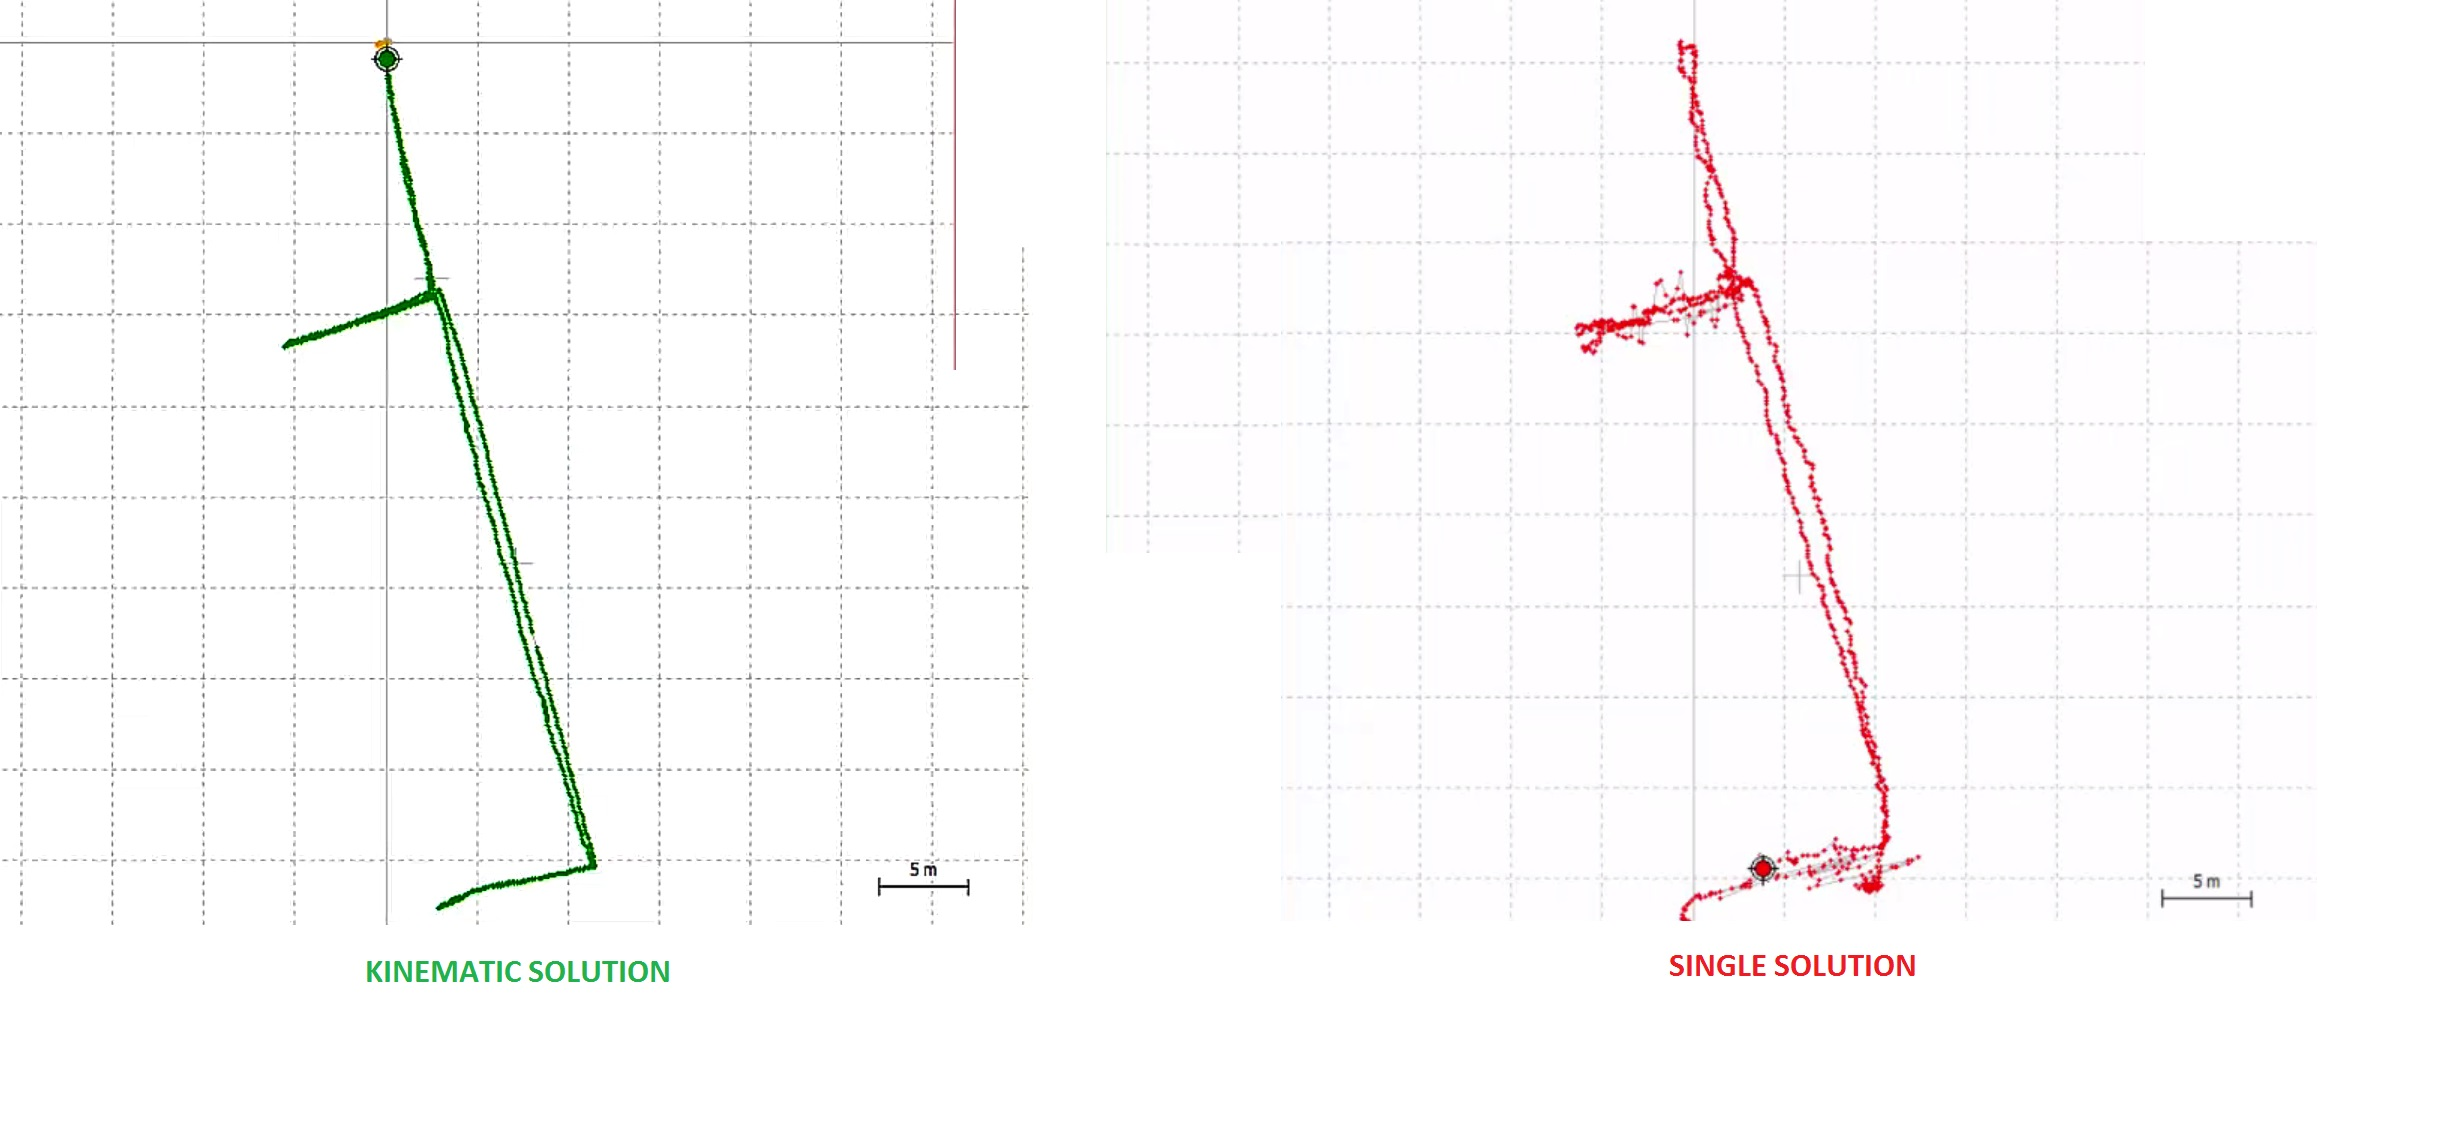
\includegraphics[width=0.95\textwidth]{Figures/MovimientosPrueba}
\caption[Pruebas de rendimiento.]{Pruebas de rendimiento}
\label{fig:Pruebas}
\end{figure}

La BeagleBone Black no presentó ningún inconveniente tanto de consumo de energía como de recursos durante la realización de las rutinas, pudiendo otorgar la solución de posicionamiento tras el procesado de forma óptima.\\

Como consecuencia, se garantiza que la información de posicionamiento del equipo que cuente con un GPS funcionando en modo Real-Time Kinematics será precisa y estable, permitiendo así que sea viable el aplicar control evitando lecturas de baja confiabilidad en la retroalimentación durante el sensado de coordenadas.